\chapter{数学的知識}
\label{chap:数学的知識}

\section{表記}

本書では基本的に実数しか扱いません.
そのため断りのない限り,実数が使われていることを前提とします.
表記としては,スカラーを$a \in \mathbb{R}$,$N$次元のベクトルを${\bf a} \in \mathbb{R}^{N}$,$N \times M$の行列を$A \in \mathbb{R}^{N \times M}$と表記します.
また単位行列をよく用いますが,次元をわかりやすくするために添え字を付けます.
例えば$N$次元の単位行列は$I_{N}$と示します.













\section{ヤコビアン}

本書では主に{\bf 最適化}(Optimization)を利用していきます.
最適化とは,ある変数${\bf x} = \left( x_{1} ~ \cdots ~ x_{N} \right)^{\top} \in \mathbb{R}^{N}$に従う関数$f({\bf x})$(最適化に使われる関数はよく{\bf コスト関数}(Cost Function)と呼ばれます)が定義されたときに,$f$の値を最小化(もしくは最大化)させること,またそれに対応する変数${\bf x}$を求めることになります.
最適化を行う方法には様々な方法がありますが,基本となることは,関数の勾配を求めることになり,これは式(\ref{eq:scholar_function_jacobian})で定義されます.
%
\begin{align}
  \frac{ \partial f({\bf x}) }{ \partial {\bf x} } =
  \left( \begin{matrix}
    \frac{ \partial f({\bf x}) }{ \partial x_{1} } &
    \cdots                                         &
    \frac{ \partial f({\bf x}) }{ \partial x_{N} }
  \end{matrix} \right)
  \label{eq:scholar_function_jacobian}
\end{align}
%
なお,関数を引数であるベクトルで偏微分した結果は,{\bf ヤコビアン}(Jacobian)と呼ばれます.
ベクトル関数${\bf f}({\bf x}) = \left( f_{1} \left( {\bf x} \right) ~ \cdots ~ f_{M} \left( {\bf x} \right) \right)^{\top} \in \mathbb{R}^{M}$に関してもヤコビアンを定めることができ,これは式(\ref{eq:vector_function_jacobian})で表すことができます.
%
\begin{align}
  \frac{ \partial {\bf f} \left( {\bf x} \right) }{ \partial {\bf x} } =
  \left( \begin{matrix}
    \frac{ \partial f_{1} \left( {\bf x} \right) }{ \partial x_{1} } &
    \cdots                                             &
    \frac{ \partial f_{1} \left( {\bf x} \right) }{ \partial x_{N} } \\
    %
    \vdots                                             &
    \ddots                                             &
    \vdots                                             \\
    %
    \frac{ \partial f_{M} \left( {\bf x} \right) }{ \partial x_{1} } &
    \cdots                                             &
    \frac{ \partial f_{M} \left( {\bf x} \right) }{ \partial x_{N} } \\
  \end{matrix} \right)
  \label{eq:vector_function_jacobian}
\end{align}
%
なお本書では,基本的にヤコビアンを$J$と表記します.

ヤコビアンの計算は基本的に式(\ref{eq:scholar_function_jacobian}),(\ref{eq:vector_function_jacobian})に示す定義に従って行いますが,少し異なった方法でも導出することが可能であり,本書では基本的にこの方法を用いてヤコビアンを求めていきます.
まず,関数$f \left( {\bf x} \right)$を$\delta {\bf x}$だけ変化させた結果をテイラー展開を用いて近似します.
%
\begin{align}
  f \left( {\bf x} + \delta {\bf x} \right) \simeq
  f \left( {\bf x} \right) + 
  J \delta {\bf x} + 
  \frac{1}{2} \delta {\bf x}^{\top} H \delta {\bf x}
  \label{eq:taylor_expansion_approximation_2nd_order}
\end{align}
%
なお$H = \partial^{2} f \left( {\bf x} \right) / \partial {\bf x}^{2}$であり,これは{\bf ヘッセ行列}(Hessian)と呼ばれます.
ここで,2次の微小量を無視し,式(\ref{eq:taylor_expansion_approximation_2nd_order})の両辺が等しいと仮定すると,次式が得られます.
%
\begin{align}
  f \left( {\bf x} + \delta {\bf x} \right) - f \left( {\bf x} \right) = J \delta {\bf x}
  \label{eq:jacobian_difference}
\end{align}
%
すなわち,$f \left( {\bf x} + \delta {\bf x} \right)$と$f \left( {\bf x} \right)$の差分を$J \delta {\bf x}$という形で記述できるとヤコビアンを求めることができます.

例えば,$f \left( x \right) = x^{2}$という簡単な例を考えてみます.
この関数のヤコビアン\footnote{正確には引数がスカラーなので導関数と呼ぶのが一般的ですが,1次元の場合のヤコビアンと形式的に見なすことができます.}は$\partial x^{2} / \partial x = 2x$となりますが,式(\ref{eq:jacobian_difference})に示す方法でヤコビアンを求めてみます.
%
\begin{align}
  \begin{split}
    (x + \delta x)^{2} - x^{2}
    = & x^{2} + 2 x \delta x + \delta x^{2} - x^{2} \\
    = & 2 x \delta x
  \end{split}
  \label{eq:jacobian_difference_example}
\end{align}
%
ただし,$\delta x^{2} \simeq 0$として2次の微小量を無視しました.  
式(\ref{eq:jacobian_difference_example})に示すように,$f \left( x \right) = x^{2}$のヤコビアンを正しく求めることができました.
この方法を用いると,関数を直接微分しなくても,ヤコビアンを求めることができます\footnote{ここで得られるヤコビアンは,関数をテイラー展開し,2次以上の微小項を無視することで得られる1次近似により得られたものです.$\delta x \to 0$ の極限では,理論的な微分(導関数)と一致しますが,有限の差分を用いる場合は数値的な近似値となります.}.













\section{ガウス・ニュートン法}
\label{subsec:gauss-newton_method}

本書で扱う問題は,度々最適化問題に帰着されます.
最適化問題を解く際に用いられる方法は様々ありますが,本書では{\bf ガウス・ニュートン法}(Gauss-Newton Method)を主に用います.

ガウス・ニュートン法を考えるにあたり,まず状態変数${\bf x} \in \mathbb{R}^{N}$,およびこの状態に依存する{\bf 残差}(Residual)(もしくは残差ベクトル)${\bf r} \left( {\bf x} \right) \in \mathbb{R}^{M}$を導入します.
今,複数の残差ベクトルを用いて,以下のコスト関数を定義します.
%
\begin{align}
  E \left( {\bf x} \right) = \sum_{i} \| {\bf r}_{i} \left( {\bf x} \right) \|_{2}^{2} \in \mathbb{R}
\end{align}
%
ここで$\| \cdot \|_{2}^{2}$は,ベクトルのユーグリッドノルムの2乗を計算する操作です.
そして,コスト関数を最小化する状態を以下のように定義します.
%
\begin{align}
  {\bf x}^{*} = \argmin_{ {\bf x} } E \left( {\bf x} \right)
\end{align}
%
これは,${\bf x}$の定義域においてコスト関数 $E \left( {\bf x} \right)$を最小にするような状態${\bf x}^{*}$を求めることを意味します.
このような解は,{\bf 最適解}(Optimal Solution)と呼ばれます.

ガウス・ニュートン法による最適化を考えるにあたり,まず残差ベクトルを1次のテイラー展開で近似することを考えます.
%
\begin{align}
  {\bf r} \left( {\bf x} + \delta {\bf x} \right) \simeq {\bf r} \left( {\bf x} \right) + J \delta {\bf x}
  \label{eq:error_vector_taylor}
\end{align}
%
ここで$J$は残差ベクトル${\bf r}$の状態ベクトル${\bf x}$に関するヤコビアン$\partial {\bf r} / \partial {\bf x} \in \mathbb{R}^{M \times N}$になります.
次に,式(\ref{eq:error_vector_taylor})の近似された残差ベクトルの2乗ノルムを考えます.
%
\begin{align}
  \begin{split}
    \left( {\bf r} + J \delta {\bf x} \right)^{\top} \left( {\bf r} + J \delta {\bf x} \right)
    %
    = & \left( {\bf r}^{\top} + \delta {\bf x}^{\top} J^{\top} \right) \left( {\bf r} + J \delta {\bf x} \right) \\
    %
    = & {\bf r}^{\top} {\bf r} + {\bf r}^{\top} J \delta {\bf x} + \delta {\bf x}^{\top} J^{\top} {\bf r} + \delta {\bf x}^{\top} J^{\top} J \delta {\bf x} \\
    %
    = & {\bf r}^{\top} {\bf r} + 2 \delta {\bf x}^{\top} J^{\top} {\bf r} + \delta {\bf x}^{\top} J^{\top} J \delta {\bf x}
  \end{split}
  \label{eq:error_vector_taylor_sq_norm}
\end{align}
%
なお,${\bf r}^{\top} J \delta {\bf x} = \delta {\bf x}^{\top} J^{\top} {\bf r}$を用いています.

続いて,式(\ref{eq:error_vector_taylor_sq_norm})を$\delta {\bf x}$の関数$f \left( \delta {\bf x} \right)$とみなして,$\delta {\bf x}$で偏微分します.
%
\begin{align}
  \frac{ \partial f \left( \delta {\bf x} \right) }{ \partial \delta {\bf x} } = 2 J^{\top} {\bf r} + 2 J^{\top} J \delta {\bf x}
  \label{eq:error_vector_taylor_sq_norm_partial}
\end{align}
%
そして,式(\ref{eq:error_vector_taylor_sq_norm_partial})が${\bf 0}$になると仮定すると,次式が成り立ちます.
%
\begin{align}
  J^{\top} J \delta {\bf x} = -J^{\top} {\bf r}
  \label{eq:gauss_newton_update_value}
\end{align}

ここで,式(\ref{eq:gauss_newton_update_value})を満たす$\delta {\bf x}$について考えます.
$f \left( \delta {\bf x} \right)$は,$\delta {\bf x}$だけ状態を変化させたときの残差ベクトルを近似し,その2乗ノルムを計算したものになっています.
これを$\delta {\bf x}$に関して偏微分し,その結果を${\bf 0}$とすると,近似した残差ベクトルの2乗ノルムを最小にする$\delta {\bf x}$を求めることが可能になります.
すなわち,この操作で求められた$\delta {\bf x}$分だけ${\bf x}$を更新すると,コスト関数を減少させることができるようになります.

式(\ref{eq:error_vector_taylor_sq_norm})を導出するにあっては,1つの残差ベクトルの近似を考えましたが,実際のコスト関数では複数の残差ベクトルの2乗ノルムの和を計算しています.
そのため,状態${\bf x}$を$\delta {\bf x}$だけ変化させたコスト関数を近似する必要がありますが,これは式(\ref{eq:cost_function_taylor})のようになります.
%
\begin{align}
  E \left( {\bf x} + \delta {\bf x} \right) \simeq \sum_{i} \left( {\bf r}_{i}^{\top} {\bf r}_{i} + 2 \delta {\bf x}^{\top} J_{i}^{\top} {\bf r}_{i} + \delta {\bf x}^{\top} J_{i}^{\top} J_{i} \delta {\bf x} \right)
  \label{eq:cost_function_taylor}
\end{align}
%
そして同様に,式(\ref{eq:cost_function_taylor})を$\delta {\bf x}$で偏微分した結果を${\bf 0}$にすると,次式が得られます.
%
\begin{align}
  \sum_{i} J_{i}^{\top} J_{i} \delta {\bf x} = -\sum_{i} J_{i}^{\top} {\bf r}_{i}
  \label{eq:gauss_newton_update_sum}
\end{align}
%
ここで簡略化のため,以下のように変数を導入します.
%
\begin{align}
  \begin{gathered}
    H = \sum_{i} J_{i}^{\top} J_{i} \\
    {\bf b} = \sum_{i} J_{i}^{\top} {\bf r}_{i}
  \end{gathered}
  \label{eq:hessian_and_gradient_gauss_newton}
\end{align}
%
これにより式(\ref{eq:gauss_newton_update_sum})は$H \delta {\bf x} = -{\bf b}$と書けます.
なおこの$H$と${\bf b}$はそれぞれヘッセ行列と勾配とも呼ばれます.
ガウス・ニュートン法を用いた最適化では,$H \delta {\bf x} = -{\bf b}$を満たす$\delta {\bf x}$を得た後に,以下のように状態を更新します.
%
\begin{align}
  {\bf x} \leftarrow {\bf x} + \delta {\bf x}
  \label{eq:gauss_newton_update_vector}
\end{align}
%
なお,$H \delta {\bf x} = -{\bf b}$からは,当然$\delta {\bf x} = -H^{-1} {\bf b}$が導けますが,$H \in \mathbb{R}^{N \times N}$になるため,$N$が大きい場合には逆行列の直接的な計算が困難になります.
そのため,直接逆行列を計算することが少ないため,「$H \delta {\bf x} = -{\bf b}$を満たす$\delta {\bf x}$」という表現を用いています.
$N$が大きくない場合は,直接$H^{-1}$を計算しても実用上は問題になりません.









\section{ロバストカーネル}

最適化を実行するにあたり,残差ベクトルを複数定義しますが,誤った対応,すなわち誤対応を用いて残差ベクトルを定義してしまうと,最適化に悪影響を及ぼすことになります.
通常,誤対応によって生じる残差ベクトルのノルムは,正しい対応に比べて大きくなる傾向があります.
そのため,残差ベクトルのノルムの大きさに応じて最適化への影響を抑制することが有効です.
このような効果を実現するために,{\bf ロバストカーネル}(Robust Kernel)を導入することができます.

一般にロバストカーネルを導入したコスト関数は以下のように記述されます.
%
\begin{align}
  E \left( {\bf x} \right) = \sum_{i} \rho \left( \| {\bf r}_{i} \left( {\bf x} \right) \|_{2}^{2} \right)
  \label{eq:cost_function_robust_kernel}
\end{align}
%
式(\ref{eq:cost_function_robust_kernel})に示す$\rho \left( \cdot \right)$がロバストカーネルになります.
ロバストカーネルにも様々なものがありますが,本書では{\bf フーバー損失}(Huber Loss)を用います.
フーバー損失は以下のように定義されます.
%
\begin{align}
  \rho \left( s \right)
  =
  \begin{cases}
    s                                & {\rm if} ~ s \leq \delta^{2} \\
    2 \delta \sqrt{ s } - \delta^{2} & {\rm otherwise}
  \end{cases}
  \label{eq:huber_loss}
\end{align}
%
ここで$\delta$は任意の正の実数です.

フーバー損失を用いたガウス・ニュートン法を考えるにあたり,式(\ref{eq:error_vector_taylor_sq_norm})に示したように,残差ベクトルの微小変化${\bf r} \left( {\bf x} + \delta {\bf x} \right)$を線形近似した結果,すなわち${\bf r} \left( {\bf x} \right) + J \delta {\bf x}$に対するフーバー損失を考ます.
%
\begin{align}
  \rho \left( \left( {\bf r} + J \delta {\bf x} \right)^{\top} \left( {\bf r} + J \delta {\bf x} \right) \right)
  =
  \rho \left( {\bf r}^{\top} {\bf r} + 2 \delta {\bf x}^{\top} J^{\top} {\bf r} + \delta {\bf x}^{\top} J^{\top} J \delta {\bf x} \right)
\end{align}
%
ここで$s = {\bf r}^{\top} {\bf r} + 2 \delta {\bf x}^{\top} J^{\top} {\bf r} + \delta {\bf x}^{\top} J^{\top} J \delta {\bf x}$とします.
式(\ref{eq:huber_loss})より,$s \leq \delta^{2}$の場合は$s$がそのまま用いられるため,$s$が$\delta^{2}$より大きくなる例を考えることとし,与えられた$s$をフーバー損失に代入した結果を$\delta {\bf x}$で微分します.
%
\begin{align}
  \begin{split}
    \frac{ \partial \rho \left( s \right) }{ \partial \delta {\bf x} }
    = &
    \frac{ \partial \rho \left( s \right) }{ \partial s }
    \frac{ \partial s }{ \partial \delta {\bf x} } \\
    = &
    \frac{ \delta }{ \sqrt{s} } \left( 2 J^{T} {\bf r} + 2 J^{\top} J \delta {\bf x} \right)
  \end{split}
  \label{eq:huber_loss_diff}
\end{align}
%
そして式(\ref{eq:huber_loss_diff})が${\bf 0}$になるとすると,以下が得られます.
%
\begin{align}
  \frac{ \delta }{ \sqrt{s} } J^{\top} J \delta {\bf x} = -\frac{ \delta }{ \sqrt{s} } J^{T} {\bf r}
  \label{eq:gauss_newton_update_value_huber_loss}
\end{align}
%
式(\ref{eq:gauss_newton_update_value})と比較すると,式(\ref{eq:gauss_newton_update_value_huber_loss})では両辺に$\delta / \sqrt{s}$が表れます.
なお式(\ref{eq:gauss_newton_update_value_huber_loss})における$\delta / \sqrt{s}$は削除することができますが,実際には複数の残差ベクトルの和を考えることとなり,この値は考える残差ベクトル毎に異なる値となるため,削除せずに記述しています.

そして,式(\ref{eq:hessian_and_gradient_gauss_newton})に示したように,すべての残差ベクトルを考慮してヘッセ行列と勾配を定めると以下のようになります.
%
\begin{align}
  \begin{gathered}
    H = \sum_{i} \rho^{\prime} \left( s_{i} \right) J_{i}^{\top} J_{i} \\
    {\bf b} = \sum_{i} \rho^{\prime} \left( s_{i} \right) J_{i}^{\top} {\bf r}_{i}
  \end{gathered}
  \label{eq:hessian_and_gradient_gauss_newton_huber_loss}
\end{align}
%
なお$\rho^{\prime} \left( s \right) = \partial \rho \left( s \right) / \partial s$であり,これは式(\ref{eq:huber_loss})より以下となります.
%
\begin{align}
  \rho^{\prime} \left( s \right)
  =
  \begin{cases}
    1                             & {\rm if} ~ s \leq \delta^{2} \\
    \frac{ \delta }{ \sqrt{ s } } & {\rm otherwise}
  \end{cases}
  \label{eq:huber_loss_prime}
\end{align}
%

ただし$s = {\bf r}^{\top} {\bf r} + 2 \delta {\bf x}^{\top} J^{\top} {\bf r} + \delta {\bf x}^{\top} J^{\top} J \delta {\bf x}$としたため,このままで$\rho^{\prime} \left( \cdot \right)$が$\delta {\bf x}$に依存してしまい,ガウス・ニュートン法の線形構造が崩れて式(\ref{eq:gauss_newton_update_sum})に示すような形で状態の更新量を求められなくなってしまいます.
そこで$s_{0} = {\bf r}^{\top} {\bf r}$,$\delta s = 2 \delta {\bf x}^{\top} J^{\top} {\bf r} + \delta {\bf x}^{\top} J^{\top} J \delta {\bf x}$とし,$\rho^{\prime} \left( s \right) \simeq \rho^{\prime} \left( s_{0} \right) + \rho^{\prime \prime} \left( s_{0} \right) \delta s$として近似します.
そして,$\rho^{\prime \prime} \left( s_{0} \right) \delta s$が高次の微小量であるとみなして無視してしまい$\rho^{\prime}(s) \simeq \rho^{\prime}(s_0)$と近似してしまいます.
これにより,$\rho^{\prime} \left( s \right) \simeq \rho^{\prime} \left( s_{0} \right)$とすることができ,$\delta {\bf x}$に依存しない形となるため,ガウス・ニュートン法における線形構造を維持することができます.

最終的に,$w = \rho^{\prime} \left( {\bf r}^{\top} {\bf r} \right)$とする重みを定義し,ヘッセ行列と勾配を以下のように定めます.
%
\begin{align}
  \begin{gathered}
    H = \sum_{i} w_{i} J_{i}^{\top} J_{i} \\
    {\bf b} = \sum_{i} w_{i} J_{i}^{\top} {\bf r}_{i}
  \end{gathered}
  \label{eq:hessian_and_gradient_gauss_newton_huber_loss_weight}
\end{align}
%
これらの$H$と${\bf b}$を用いて$H \delta {\bf x} = -{\bf b}$を満たす$\delta {\bf x}$を求め,式(\ref{eq:gauss_newton_update_vector})に基づき状態更新を行うことで,フーバー損失を用いたガウス・ニュートン法による最適化を実行することができます.
フーバー損失を用いた場合のガウス・ニュートン法による状態更新の導出は少し複雑にはなりますが,実装にあたっては,単に式(\ref{eq:huber_loss_prime})に示す関数を重みとして計算してそれぞれのヘッセ行列と勾配に掛けるだけなので,非常に容易に実装することができます.
また多くの場合,フーバー損失を用いることで最適化がよりロバストになります.
















\section{リー群とリー代数}

本書では頻繁に{\bf リー群}(Lie Group)と{\bf リー代数}(Lie Algebra)を用います.
リー群やリー代数の厳密な説明は行いませんが,本書でリー群と呼んだ場合は{\bf 回転行列}(Rotation Matrix)と{\bf 剛体変換行列}(Rigid Transformation Matrix)を示すこととします.

回転行列は以下のように定義されます.
%
\begin{align}
  \{R \in \mathbb{R}^{3 \times 3} | R^{\top} R = I, {\rm det}(R) = 1\}
  \label{eq:def_SO3}
\end{align}
%
回転行列はSpecial Orthogonal Group in 3 Dimensions(${\rm SO}(3)$)とも呼ばれ,3次元空間の回転を表現することができます.
剛体変換行列は以下のように定義されます.
%
\begin{align}
  \left\{ \left( \begin{matrix} R & {\bf t} \\ {\bf 0}^{\top} & 1 \end{matrix} \right) \in \mathbb{R}^{4 \times 4} | R \in {\rm SO}(3), {\bf t} \in \mathbb{R}^{3} \right\}
  \label{eq:def_SE3}
\end{align}
%
剛体変換行列はSpecial Euclidean Group in 3 Dimensions(${\rm SE}(3)$)とも呼ばれ,3次元空間での回転を含む位置(姿勢)を表現することができます.
LIOやSLAMでは基本的に,${\rm SO}(3)$や${\rm SE}(3)$を用いて状態を表現します.
なお式(\ref{eq:def_SE3})から明らかなように,$T$を構成する変数は${\bf t}$と$R$になります.
そのため,本書ではしばしば$T = \left( R \mid {\bf t} \right)$という簡略表記を用います.

リー群を用いる利点は,回転の状態を,途中で急に値が飛んだり切り替わったりすることなく,滑らかにかつ数学的に自然な形で扱えるということです.
詳細は省きますが,このような空間を{\bf 多様体}(Manifold)と呼びます.
直感的には少し難しく感じるかもしれませんが,まずは平面上の回転,つまり$xy$平面での角度$\theta$を例に考えてみます.
角度$\theta$は通常,$0 \leq \theta < 2\pi$(あるいは$-\pi \leq \theta < \pi$)の範囲で定義されますが,$\theta = 0$と$\theta = 2\pi$は,数値としては異なるものの,回転としては同じ状態を表しています.
このような性質から,角度$\theta$による表現では,状態が不連続に見えることがあります.
しかしリー群を使えば,回転の変化を「切れ目のない空間」で表現でき,最初から最後まで滑らかに(連続的に)扱えるようになります.
また,加減算や微分といった操作も数学的に統一されたルールで行えるので,処理が一貫してスムーズになります.
しかしリー群を用いて状態を表すと,処理が少し直感的なものではなくなってしまいます.

例えばロボットの状態をあるベクトル空間で${\bf x}$と表すとします.
もしロボットの状態が$\Delta {\bf x}$だけ変化したとすると,直感的にはロボットの状態は${\bf x} + \Delta {\bf x}$という,シンプルな加算により求めることができます(ただし前述のような角度$\theta$が含まれる場合は値の範囲に中止いなければなりません).
しかし式(\ref{eq:def_SO3}),(\ref{eq:def_SE3})に示す通り,${\rm SO}(3)$や${\rm SE}(3)$には満たすべき制約があるため,同様の加算を行うとこのような制約を満たさなくなります.

例えば,3次元空間上での並進と回転を含む変化量を$\Delta T \in {\rm SE}(3)$とし,以下のように定めます.
%
\begin{align}
  \Delta T
%
  = \left( \begin{matrix}
      \Delta R       & \Delta {\bf t} \\
      {\bf 0}^{\top} & 1
    \end{matrix} \right)
\end{align}
%
ここで,$T$と$\Delta T$の単純な加算を考えると以下になります.
%
\begin{align}
  T + \Delta T
%
  = \left( \begin{matrix}
      R + \Delta R       & {\bf t} + \Delta {\bf t} \\
      {\bf 0}^{\top}     & 2
    \end{matrix} \right) \notin {\rm SE}(3)
\end{align}
%
これは明らかに式(\ref{eq:def_SE3})を満たさないため,$T + \Delta T$は剛体変換行列にはなりません.
${\rm SE}(3)$の制約を満たしたまま変化を反映させるためには,$T \Delta T$を計算します\footnote{行列の積は左右どちらから掛けるかで結果が変わるため,$\Delta T$をどちらから作用させるかが重要になりますが,本書では基本的に動作に伴う変化に関しては右作用を用います.}.
%
\begin{align}
  T \Delta T
%
  = \left( \begin{matrix}
      R \Delta R     & R \Delta {\bf t} + {\bf t} \\
      {\bf 0}^{\top} & 1
    \end{matrix} \right) \in {\rm SE}(3)
  \label{eq:se3_add}
\end{align}
%
また,$T_{1}, T_{2} \in {\rm SE}(3)$間の差分を$\Delta T$とした場合,$T_{1} \Delta T = T_{2}$となるため,$T_{1}$と$T_{2}$の間の差分は以下のように定義されます.
%
\begin{align}
  \begin{split}
    \Delta T
%
    & = T_{1}^{-1} T_{2} \\
%
    & = \left( \begin{matrix}
          R_{1}^{\top} R_{2} & R_{2} ({\bf t}_{2} - {\bf t}_{1}) \\
          {\bf 0}^{\top}     & 1
        \end{matrix} \right) \in {\rm SE}(3)
  \end{split}
  \label{eq:se3_diff}
\end{align}

式(\ref{eq:se3_add}),(\ref{eq:se3_diff})を用いれば,${\rm SE}(3)$(もしくは${\rm SO}(3)$)の空間での状態の変化を考えることができます.
しかしこれらはベクトル空間で議論される加算や減算と比較すると直感的でなく,また前節までで述べたガウス・ニュートン法が適用できる表現になっていません.
そこで,リー群を用いて表せられている状態をベクトルに対応させなれないかということを考えますが,リー群に対応したベクトル空間としてリー代数を用いることができます.
そして${\rm SO}(3)$,${\rm SE}(3)$に対応したリー代数をそれぞれ$\mathfrak{so}(3)$,$\mathfrak{se}(3)$と記述します.
$\mathfrak{so}(3)$と$\mathfrak{se}(3)$は厳密にはそれぞれ$\mathbb{R}^{3 \times 3}$と$\mathbb{R}^{4 \times 4}$の行列の集合ですが,それぞれ独立した3つと6つの実数で表現することができるため,3次元,および6次元ベクトルとして表現できます.
そして,${\rm SO}(3)$と$\mathfrak{so}(3)$,もしくは${\rm SE}(3)$と$\mathfrak{se}(3)$間を変換させる写像として,それぞれ{\bf 指数写像}(Exponential Map)と{\bf 対数写像}(Logarithm Map)があります.
%
\begin{align}
  \begin{gathered}
    \exp: \mathfrak{so}(3) \rightarrow {\rm SO}(3) \\
    \log: {\rm SO}(3) \rightarrow \mathfrak{so}(3) \\
  \end{gathered}
  \label{eq:so3_exp_log_maps}
\end{align}
%
\begin{align}
  \begin{gathered}
    \exp: \mathfrak{se}(3) \rightarrow {\rm SO}(3) \\
    \log: {\rm SO}(3) \rightarrow \mathfrak{se}(3) \\
  \end{gathered}
  \label{eq:se3_exp_log_maps}
\end{align}
%
なお,式(\ref{eq:so3_exp_log_maps})と式(\ref{eq:se3_exp_log_maps})に示す指数・対数写像はそれぞれ別物になります.
ただし,本書で使用するにあたって適宜${\rm SO}(3)$や${\rm SE}(3)$といった断りは入れないため,引数となっている変数でどちらの写像が使われているか判断します.

リー代数を用いることで,状態量がリー群を用いて表現されている場合でも,ガウス・ニュートン法などを用いた最適化を行うことができますが,リー代数を用いた最適化を述べる前に,指数写像や対数写像について解説します.
ただしこれらの写像の導出はせず,あくまで計算がどのように行われているかだけを示します.











\subsection{指数写像と対数写像}

ある3次元ベクトル$\boldsymbol \phi$に対して,式(\ref{eq:so3_exp_log_maps})に示す指数写像は以下のように定義されます.
%
\begin{align}
  \begin{gathered}
    \theta = \| \boldsymbol \phi \|_{2} \\
    %
    \exp \left( \boldsymbol \phi^{^\wedge} \right)
    =
    I_{3} +
    \frac{ \sin \theta }{ \theta } \boldsymbol \phi{^\wedge} +
    \frac{ 1 - \cos \theta }{ \theta^{2} } \left( \boldsymbol \phi{^\wedge} \right)^{2}
  \end{gathered}
  \label{eq:so3_exp_map}
\end{align}
%
ここで$\left( \cdot \right)^{\wedge}$は,3次元ベクトルを$\mathfrak{so}(3)$に変換する操作(もしくは6次元ベクトルを$\mathfrak{se}(3)$に変換する操作)であり,3次元ベクトルの場合は{\bf 反対称行列}(Skew-Symmetric Matrix)を生成する操作であるともみなせます.
%
\begin{align}
  \boldsymbol \phi^{^\wedge}
%
  = \left( \begin{matrix}
      0         & -\phi_{z} & \phi_{y} \\
      \phi_{z}  & 0         & -\phi_{x} \\
      -\phi_{y} & \phi_{x}  & 0
    \end{matrix} \right) \in \mathfrak{so}(3)
  \label{eq:skew_symmetric_matrix}
\end{align}
%
少し話が逸れますが,反対称行列の持つ性質として,${\bf a}^{^\wedge} {\bf b} = -{\bf b}^{^\wedge} {\bf a}$というものがあります(ただし${\bf a}, {\bf b} \in \mathbb{R}^{3}$です).
%
\begin{align}
  \begin{split}
    {\bf a}^{^\wedge} {\bf b}
%
    & = \left( \begin{matrix}
          -a_{z} b_{y} + a_{y} b_{z} \\
           a_{z} b_{x} - a_{x} b_{z} \\
          -a_{y} b_{x} + a_{x} b_{y}
        \end{matrix} \right) \\
%
    & = \left( \begin{matrix}
          0      &  b_{z} & -b_{y} \\
          -b_{z} & 0      & b_{x} \\
          b_{y}  & -b_{x} & 0
        \end{matrix} \right)
        \left( \begin{matrix}
          a_{x} \\
          a_{y} \\
          a_{z}
        \end{matrix} \right) \\
%
     & = -{\bf b}^{\wedge} {\bf a} 
  \end{split}
\end{align}
%
この性質は,後ほどの実装でヤコビアンを計算するときに用います.

また,式(\ref{eq:so3_exp_log_maps})に示す対数写像は以下のように定義されます.
%
\begin{align}
  \begin{gathered}
    \theta = \arccos \left( \frac{{\rm tr}(R) - 1}{ 2 } \right) \\
    %
    \log( R ) = \frac{ \theta }{ 2 \sin \theta } \left( R - R^{\top} \right)
  \end{gathered}
  \label{eq:so3_log_map}
\end{align}
%
なお$\log \left( R \right) = \boldsymbol \phi^{\wedge} \in \mathfrak{so}(3)$となるため,この反対称行列から3次元ベクトル$\boldsymbol \phi = \left( \phi_{x} ~ \phi_{y} ~ \phi_{z} \right)^{\top}$を取り出す操作を以下のように定義します.
%
\begin{align}
  \boldsymbol \phi = \left( \boldsymbol \phi^{\wedge} \right)^{\vee}
\end{align}
%
後に示しますが,$\mathfrak{se}(3)$から6次元ベクトルを取り出す操作も同様に$\left( \cdot \right)^{\vee}$と表記します.

式(\ref{eq:so3_exp_map}),(\ref{eq:so3_log_map})では,それぞれ$\theta$が分母に表れるため,$\theta \ll 1$の場合計算が不安定になります.
そのため$\theta \ll 1$の場合には,以下のように近似して計算を行います.
%
\begin{align}
  \begin{gathered}
    \exp \left( \boldsymbol \phi^{\wedge} \right) \simeq I_{3} + \boldsymbol \phi^{\wedge} + \frac{1}{2} \left( \boldsymbol \phi^{\wedge} \right)^{2} \\
%
    \log \left( R \right) \simeq \frac{1}{2} \left( R - R^{\top} \right)
  \end{gathered}
  \label{eq:so3_exp_log_maps_approx}
\end{align}


次に,${\rm SE}(3)$に関する指数・対数写像を考えるにあたり,$\boldsymbol \xi = \left( {\bf v}^{\top} ~ \boldsymbol \phi^{\top} \right)^{\top}$となる6次元ベクトルを定義します.
そしてこの6次元ベクトルを$\mathfrak{se}(3)$とする操作を以下のように定めます\footnote{式(\ref{eq:skew_symmetric_matrix})にて$\left( \cdot \right)^{\wedge}$を3次元ベクトルに対応する反対称行列を生成する操作としていますが,6次元ベクトルの場合は式(\ref{eq:se3_wedge})に示すように$\mathfrak{se}(3)$を生成する操作として扱います.}.
%
\begin{align}
  \boldsymbol \xi^{\wedge} = \left( \begin{matrix}
    \boldsymbol \phi^{\wedge} & {\bf v} \\
    {\bf 0}^{\top}            & 0
  \end{matrix} \right) \in \mathfrak{se}(3)
  \label{eq:se3_wedge}
\end{align}
%
ここで$\boldsymbol \phi^{\wedge}$は式(\ref{eq:skew_symmetric_matrix})に示す反対称行列を返す操作になります.
式(\ref{eq:se3_wedge})を用いて,式(\ref{eq:se3_exp_log_maps})に示す指数写像は以下のように定義されます.
%
\begin{align}
  \exp \left( \boldsymbol \xi^{\wedge} \right) = \left( \begin{matrix}
    \exp \left( \boldsymbol \phi^{\wedge} \right) & J_{l} \left( \boldsymbol \phi^{\wedge} \right) {\bf v} \\
    {\bf 0}^{\top}                                & 1
  \end{matrix} \right)
  \label{eq:se3_exp_map}
\end{align}
%
なお$\exp \left( \boldsymbol \phi^{\wedge} \right)$は式(\ref{eq:so3_exp_map})に示すものであり,$J_{l} \left( \cdot \right)$は左ヤコビアンとして以下のように定義されます.
%
\begin{align}
  J_{l} \left( \boldsymbol \phi^{\wedge} \right)
  =
  I_{3} +
  \frac{ 1 - \cos \theta }{ \theta^{2} } \boldsymbol \phi^{\wedge} +
  \frac{ \theta - \sin \theta }{ \theta^{3} } \left( \boldsymbol \phi^{\wedge} \right)^{2}
  \label{eq:so3_left_jacobian}
\end{align}
%
ただし,$\theta = \| \boldsymbol \phi \|_{2}$になります.

式(\ref{eq:se3_exp_log_maps})に示す対数写像は以下のように定義されます.
%
\begin{align}
  \log \left( T \right) = \left( \begin{matrix}
    \boldsymbol \phi^{\wedge} & J_{l}^{-1} \left( \boldsymbol \phi \right) {\bf t} \\
    {\bf 0}^{\top}            & 0
  \end{matrix} \right)
  \label{eq:se3_log_map}
\end{align}
%
ここで$J_{l}^{-1} \left( \cdot \right)$は左ヤコビアンの逆行列であり,以下のように定義されます.
%
\begin{align}
  J_{l}^{-1} \left( \boldsymbol \phi \right)
  =
  I_{3} -
  \frac{1}{2} \boldsymbol \phi^{\wedge} + 
  \left( \frac{1}{ \theta^{2} } - \frac{ 1 + \cos \theta }{ 2 \theta \sin \theta } \right) \left( \boldsymbol \phi^{\wedge} \right)^{2}
  \label{eq:so3_left_jacobian_inverse}
\end{align}
%
ただし同様に$\theta = \| \boldsymbol \phi \|_{2}$となります.
なお$\log \left( T \right) \in \mathfrak{se}(3)$は$\mathbb{R}^{4 \times 4}$の行列であるため,ここから6次元のベクトル$\boldsymbol \xi$を取得する操作を以下のように定めます.
%
\begin{align}
  \begin{split}
    \boldsymbol \xi
%
    = & \left( \begin{matrix}
      J_{l}^{-1} \left( \boldsymbol \phi \right) {\bf t} \\
      \boldsymbol \phi
    \end{matrix} \right) \\
%
    = & \left( \log \left( T \right) \right)^{\vee}
  \end{split}
\end{align}
%
ただし$\boldsymbol \phi = \left( \log \left( R \right) \right)^{\vee}$となります.

なお式(\ref{eq:so3_left_jacobian}),(\ref{eq:so3_left_jacobian_inverse})においても,$\theta$が分母に含まれます.
そのため,$\theta \ll 1$となる場合は,式(\ref{eq:so3_exp_log_maps_approx})に示すように,数値計算の不安定さを回避するために近似計算を行う必要があります.











\subsection{リー代数を介した状態更新}

前述の通り,対数写像を用いることでリー群の元をリー代数の元に写像することができ,ベクトル空間上での最適化を適用することが可能となります.
これにより,例えばガウス・ニュートン法のような非線形最適化アルゴリズムをリー群に対して適用することができます.
ただし,最終的な状態はリー群上の元として表現されるため,リー代数を介した状態更新の方法を整理しておきます.
なお以下では ${\rm SE}(3)$ を対象に議論を進めますが,${\rm SO}(3)$ に関しても同様の考え方が適用されます.

例えばガウス・ニュートン法などを用いて,状態$T \in {\rm SE}(3)$に対するリー代数上での更新量$\delta \boldsymbol \xi \in \mathbb{R}^6$が求められたとします.
この更新量は,指数写像を介してリー群の元に変換され,実際の状態更新は以下のように行われます.
%
\begin{align}
  T \leftarrow \exp \left( \delta \boldsymbol \xi^{\wedge} \right) T
  \label{eq:se3_update_left}
\end{align}
%
この操作は,リー代数の元である$\delta \boldsymbol \xi$を,リー群の元$T$に加算している操作ともみなすことができ,式(\ref{eq:gauss_newton_update_vector})と対応させて以下のように書くこともあります.
%
\begin{align}
  T \leftarrow T \boxplus \delta \boldsymbol \xi
  \label{eq:se3_update_left_boxplus}
\end{align}
%
なお式(\ref{eq:se3_update_left})では状態更新のために$\exp \left( \delta \boldsymbol \xi^{\wedge} \right)$を左から掛けていますが,これは最適化計算のときの勾配を考えるときに,リー群の左からの摂動に対する残差の変化を考えているためです.
もし右からの摂動を考える場合には$\exp \left( \delta \boldsymbol \xi^{\wedge} \right)$を右から掛ける必要があるため注意が必要になります.

もし$\boldsymbol \xi = \left( \log \left( T \right) \right)^{\vee}$と表されると仮定した場合,リー代数上での新たな状態ベクトルは$\boldsymbol \xi + \delta \boldsymbol \xi$となります.
ここで$\delta \boldsymbol \xi$が微小変化であるとした上で{\bf Baker-Campbell-Hausdorff}(BCH)展開を考えると,以下の近似式を得ることができます.
%
\begin{align}
  \begin{split}
    \exp\left( (\boldsymbol \xi + \delta \boldsymbol \xi)^{\wedge} \right)
    \simeq & 
    \exp(\delta \boldsymbol \xi^{\wedge}) \exp(\boldsymbol \xi^{\wedge}) \\
    = &
    \exp(\delta \boldsymbol \xi^{\wedge}) T
  \end{split}
\end{align}
%
よって式(\ref{eq:se3_update_left})に示すように状態更新を行うことができることが確認できます.













\subsection{リー群を用いたヤコビアンの計算}

\ref{subsec:gauss-newton_method}項で述べた通り,ガウス・ニュートン法を利用するにあたってはヤコビアンを導出することが重要になります.
例えば今,$T \in {\rm SE}(3)$に依存する残差ベクトル${\bf r} \in \mathbb{R}^{N}$があるとします.
このヤコビアンを求めるためには,次式を満たす$J$を求めれば良いことになります.
%
\begin{align}
  {\bf r} \left( \exp \left( \delta \boldsymbol \xi^{\wedge} \right) T \right) - {\bf r}(T)
= J \delta \boldsymbol \xi
\end{align}
%
なお$J \in \mathbb{R}^{N \times 6}$(${\bf r}\left( R \right) \in \mathbb{R}^{N}, R \in {\rm SO}(3)$の場合は$\mathbb{R}^{N \times 3}$)となります.
実際に残差ベクトルを定めてヤコビアンを求める例は,次章以降で述べています.

また残差ベクトルを微分するにあたり,リー群の元同士での微分を行うことがあります.
これを考えるために,一例としてシンプルな$\partial T / \partial T$について考えてみます.
この場合は,以下の式を満たすヤコビアン$J$を求めれば良いことになります.
%
\begin{align}
  T^{-1} \left( \exp \left( \delta \boldsymbol \xi^{\wedge} \right) T \right) = I_{4} + \left( J \delta \boldsymbol \xi \right)^{\wedge}
  \label{eq:dT_dT}
\end{align}
%
これは式(\ref{eq:se3_diff})に示すような,$\exp \left( \delta \boldsymbol \xi^{\wedge} \right) T$と$T$の差分を考えていることになり,特に$T^{-1} T = I_{4}$であることから,リー群の恒等元周りでの微小変動を考えていることになります.
そのためベクトル空間で$f \left( {\bf x} + \delta {\bf x} \right) - f \left( {\bf x} \right) = J \delta {\bf x}$という式を考えていることと等価になります.
ただし$J \delta \boldsymbol \xi$は6次元のベクトルとなるため,そのままでは$I_{4}$に加算することができないので,$\left( \cdot \right)^{\wedge}$作用により対応する$\mathfrak{se}(3)$に変換していることに注意してください.
そして,$T^{-1} \exp \left( \delta \boldsymbol \xi^{\wedge} \right) T$は以下のように書くことができます.
%
\begin{align}
  T^{-1} \exp \left( \delta \boldsymbol \xi^{\wedge} \right) T = \exp \left( \left( \operatorname{Ad}_{T^{-1}} \delta \boldsymbol \xi \right)^{\wedge} \right)
\end{align}
%
ここで$\operatorname{Ad}_{T} \in \mathbb{R}^{6 \times 6}$は{\bf 随伴作用素}(Adjoint)と呼ばれます(詳細な定義は次項で述べます).
ここで$\delta \boldsymbol \xi$が微小変動であることを考慮すると,以下のように近似することができます.
%
\begin{align}
  \exp \left( \left( \operatorname{Ad}_{T^{-1}} \delta \boldsymbol \xi \right)^{\wedge} \right) \simeq I_{4} + \left( \operatorname{Ad}_{T^{-1}} \delta \boldsymbol \xi \right)^{\wedge}
  \label{eq:dT_dT_Ad}
\end{align}
%
式(\ref{eq:dT_dT}),(\ref{eq:dT_dT_Ad})を比較すると,$J = \operatorname{Ad}_{T^{-1}}$となることがわかり,これが$\partial T / \partial T$の結果となります.







\subsection{随伴作用素}

随伴作用素とは,以下の式を満たすものとなります.
%
\begin{align}
  \begin{gathered}
    \left( \operatorname{Ad}_{R} \boldsymbol \phi \right)^{\wedge} = R \boldsymbol \phi^{\wedge} R^{\top} \\
%
    \left( \operatorname{Ad}_{T} \boldsymbol \xi \right)^{\wedge} = T \boldsymbol \xi^{\wedge} T^{-1}
  \end{gathered}
  \label{eq:adjoint}
\end{align}
%
ただし$\boldsymbol \phi \in \mathbb{R}^{3}$,$\boldsymbol \xi \in \mathbb{R}^{6}$になります.
詳細な導出方法に関しては省きますが,それぞれの随伴作用素は以下のように定義されます.
%
\begin{align}
  \operatorname{Ad}_{R} = R
  \label{eq:adjoint_so3}
\end{align}
%
\begin{align}
  \operatorname{Ad}_{T} = \left( \begin{matrix}
    R & {\bf t}^{\wedge} R \\
    0 & R
  \end{matrix} \right)
  \label{eq:adjoint_se3}
\end{align}







\section{座標系とその表記}

\begin{figure}[!t]
  \centering
  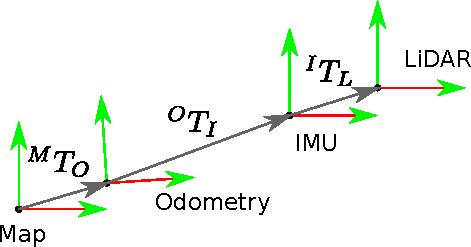
\includegraphics[width=0.4\textwidth]{../figs/frames.pdf}
  \caption{Coordinate frames employed in this work.}
  \label{fig:frames}
\end{figure}

本書で扱う座標系は主に図\ref{fig:frames}に示すように地図,オドメトリ,IMU,LiDARの4つの座標になります.
それぞれの座標は,$M$,$O$,$I$,$L$の添字により表すこととします.
例えばある点${\bf p}$がそれぞれの座標で定められる場合,左上に添え字を置きそれぞれ${}^{M}{\bf p}$,${}^{O}{\bf p}$,${}^{I}{\bf p}$,${}^{L}{\bf p}$と表します.
またある点の座標変換(Source $S$からTarget $T$への変換)を考えるとき,以下のどちらかを用いて表します.
%
\begin{align}
  \begin{gathered}
    {}^{T}{\bf p} = {}^{T}R_{S} {}^{S}{\bf p} + {}^{T}{\bf t}_{S} \\
%
    {}^{T}{\bf p} = {}^{T}T_{S} {}^{S}{\bf p}
  \end{gathered}
  \label{eq:point_transformation}
\end{align}
%
ただし${\rm SE}(3)$を用いるときは${\bf p} \in \mathbb{R}^{4}$となり,4要素目には1が入ることになります.

例えば,IMU座標からオドメトリ座標に点を変換する場合は,${}^{O}{\bf p} = {}^{O}R_{I} {}^{I}{\bf p} + {}^{O}{\bf t}_{I}$,もしくは${}^{O}{\bf p} = {}^{O}T_{I} {}^{I}{\bf p}$と表記します.
また,もしIMU座標から地図座標への変換を直接考えるときは,以下のどちらかを用います.
%
\begin{align}
  \begin{gathered}
    {}^{M}{\bf p} = {}^{M}R_{O} \left( {}^{O}R_{I} {}^{I}{\bf p} + {}^{O}{\bf t}_{I} \right) + {}^{M}{\bf t}_{O}\\
%
    {}^{M}{\bf p} = {}^{M}T_{O} {}^{O}T_{I} {}^{I}{\bf p}
  \end{gathered}
  \label{eq:point_transformation_synthesis}
\end{align}
%
ただし,${}^{M}T_{I} = {}^{M}T_{O} {}^{O}T_{I}$とし,またこれに対応する並進ベクトルと回転行列を${}^{M}{\bf t}_{I}$,${}^{M}R_{I}$とすれば,式(\ref{eq:point_transformation_synthesis})は式(\ref{eq:point_transformation})のように1つの変換にまとめて書くこともできます.

なお図\ref{fig:frames}に示すそれぞれの座標変換ですが,基本的には,IMUとLiDAR間の変換${}^{I}T_{L}$は静的であるため事前にキャリブレーションで求め,LIOが${}^{O}T_{I}$,SLAM(もしくは自己位置推定)が${}^{M}T_{O}$を求めることになります.
ただし,${}^{I}T_{L}$もオンラインで最適化することもできます.
またSLAMや自己位置推定を使わずに,LIOが直接地図座標への変換を求めると仮定する場合もあるため,図\ref{fig:frames}に示す座標を必ず守らなければならないということではありません.


